\documentclass[UTF8]{ctexbook}
\usepackage{amsmath}
\usepackage{amsfonts}
\usepackage{amssymb}
\usepackage[a5paper, inner=18mm, outer=15mm, top=15mm, bottom=18mm]{geometry}
\usepackage{graphicx}
\usepackage{caption}
% \usepackage{emoji}
\usepackage{multicol}
\usepackage{xcolor}
\usepackage{fontspec}
\usepackage{url}
\usepackage{hyperref}
\usepackage[capitalize]{cleveref}

\hypersetup{
    pdfauthor={Gy-ers},
    pdftitle={广雅生存手册（高中版）},
    pdfcreator={LuaLaTeX},
    pdfproducer={LaTeX}
}

% \setCJKfamilyfont{hei}{SimHei}[Renderer=Basic,AutoFakeBold=3]
% \renewcommand{\heiti}{\CJKfamily{hei}}

\setCJKmainfont[
     Path=/usr/share/fonts/truetype/,
     Filename=SimSun.ttc,
     AutoFakeBold=2.8,  % 宋体自身加粗，不用simhei顶替粗体
     AutoFakeSlant=0.2
]{SimSun}
 % 无衬线黑体（\heiti、标题），开启伪粗体解决加粗方块
 \setCJKsansfont[
     Path=/usr/share/fonts/truetype/,
     Filename=simhei.ttf,
     AutoFakeBold=3.0,  % 关键：给SimHei生成模拟粗体
     AutoFakeSlant=0.2
]{SimHei}

% 彻底放弃 Emoji 了，有能耐的人再搞吧...
% \newfontfamily\emojifont{Noto Color Emoji}{Renderer=HarfBuzz}
% \DeclareTextFontCommand{\textemoji}{\emojifont}

\numberwithin{figure}{section}
\numberwithin{table}{section}

\crefformat{figure}{\heiti {图#2#1#3}}
\crefformat{table}{\heiti {表#2#1#3}}
\crefformat{chapter}{\heiti {第#2#1#3章}}
\crefformat{section}{\heiti {第#2#1#3节}}
\crefformat{subsection}{\heiti {第#2#1#3节}}
\renewcommand{\tablename}{\heiti 表}
\renewcommand{\figurename}{\heiti 图}

\graphicspath{{../pics/}}


\title{\heiti \zihao{1} 广雅生存手册\\（高中）}
\author{\textsf{GY-ers}}
\date{\today 更新}

\begin{document}
\maketitle

\frontmatter

\chapter{前言}

目前来说，这个项目是挂在GitHub上的，地址为\url{https://github.com/druvis1023/GY-Guide.git}，所有人都可以参与编写，贡献自己的一份力量。

写这个，主要是为了广雅的学弟学妹们能够更好地了解广雅。目前暂时没有想好有什么内容可以写。这本书的内容\textbf{仅供参考}，毕竟每个年级的制度会根据级长的要求而有所不同，比如说24级晚修只需19点到班，而25级的级长18：40左右就在走廊守人…毕竟他们18：50开始晚修。

这本《广雅生存手册（高中）》仅仅适用于花都校区，并且，不是广雅官方写的，而是一群想要把自己的一些踩过的坑、碰到的雷让学弟学妹避开的同学们一起编写的，因此也会比官方更敢说。不仅如此，还会教授一些小秘密。

如果你也有一些避雷或者是有意思的内容，欢迎填写问卷、在GitHub提交Issue或者直接发邮件给本文主要执笔者\href{mailto:druvis1023@hotmail.com}{druvis1023@hotmail.com}，来为这本《广雅生存手册（高中）》添砖加瓦！

如果你是第一次住宿，那么，这里将会告诉你有什么需要准备的

\section*{生活用品}
\begin{multicols}{3}
\begin{itemize}
    \item 行李箱
    \item 书包
    \item 梳子（选带）
    \item 镜子（选带）
    \item 发夹 \& 发圈（选带）
    \item 衣架
    \item 毛巾
    \item 卫生纸
    \item 卫生巾（选带）
    \item 伞
    \item 吹风机
    \item 水杯
    \item 夹子
    \item 洗面奶（选带）
    \item 沐浴露 / 香皂
    \item 洗发水
    \item 护发素（选带）
    \item 洗衣液
    \item 灯（选带）
    \item 牙膏 + 牙刷 + 刷牙杯
    \item 盆 + 桶
\end{itemize}
\end{multicols}

\section*{床上用品}
\begin{multicols}{3}
\begin{itemize}
    \item 床上四件套（床单、被套、枕套）
    \item 床垫、枕头、被子
    \item 蚊帐
    \item 凉席（选带）
\end{itemize}
\end{multicols}

\section*{衣物}
\begin{multicols}{3}
\begin{itemize}
    \item 校服短袖（两套及以上）
    \item 短裤（两条及以上）
    \item 长裤（按需带）
    \item 外套（按需带）
    \item 班服（选带）
    \item 袜子
    \item 内衣裤
    \item 拖鞋
\end{itemize}
\end{multicols}

\section*{文具\&书籍}
\begin{multicols}{3}
\begin{itemize}
    \item 笔袋 / 笔盒
    \item 黑、蓝、红笔
    \item 2B 铅笔
    \item 橡皮
    \item 荧光笔
    \item 订书机 + 订书钉（非必要）
    \item 笔记本
    \item 便利贴
    \item 试卷夹
    \item 文件袋（选带）
    \item 胶带（双面胶 / 透明胶）（非必要）
    \item 书袋
    \item 名著
    \item 作业
    \item 练习册
    \item 全解（非必要）
\end{itemize}
\end{multicols}

有了这个清单，收拾东西应该不会有遗漏了吧（笑），希望第一周能过得愉快。



\tableofcontents

\mainmatter

\chapter{广雅的学习}
\label{chap:study}

  \section{关于分科}
    相信很多高一新入学的学生都对自己高一下的选科、分科有很多疑惑。
  
  \section{打印在读证明}
    在读证明有很大的用处，可以向 Jetbrains 申请学生优惠和一些学生免费，也可以去广州大剧院半价看戏。打印在读证明比较方便的方式为自行打印，有两台机可以打印：一楼书吧和四楼高三书吧。如\cref{fig:prove1}为高三书吧的打印机
    \begin{figure}[ht]
      \centering
      \begin{minipage}{0.45\textwidth}
        \centering
        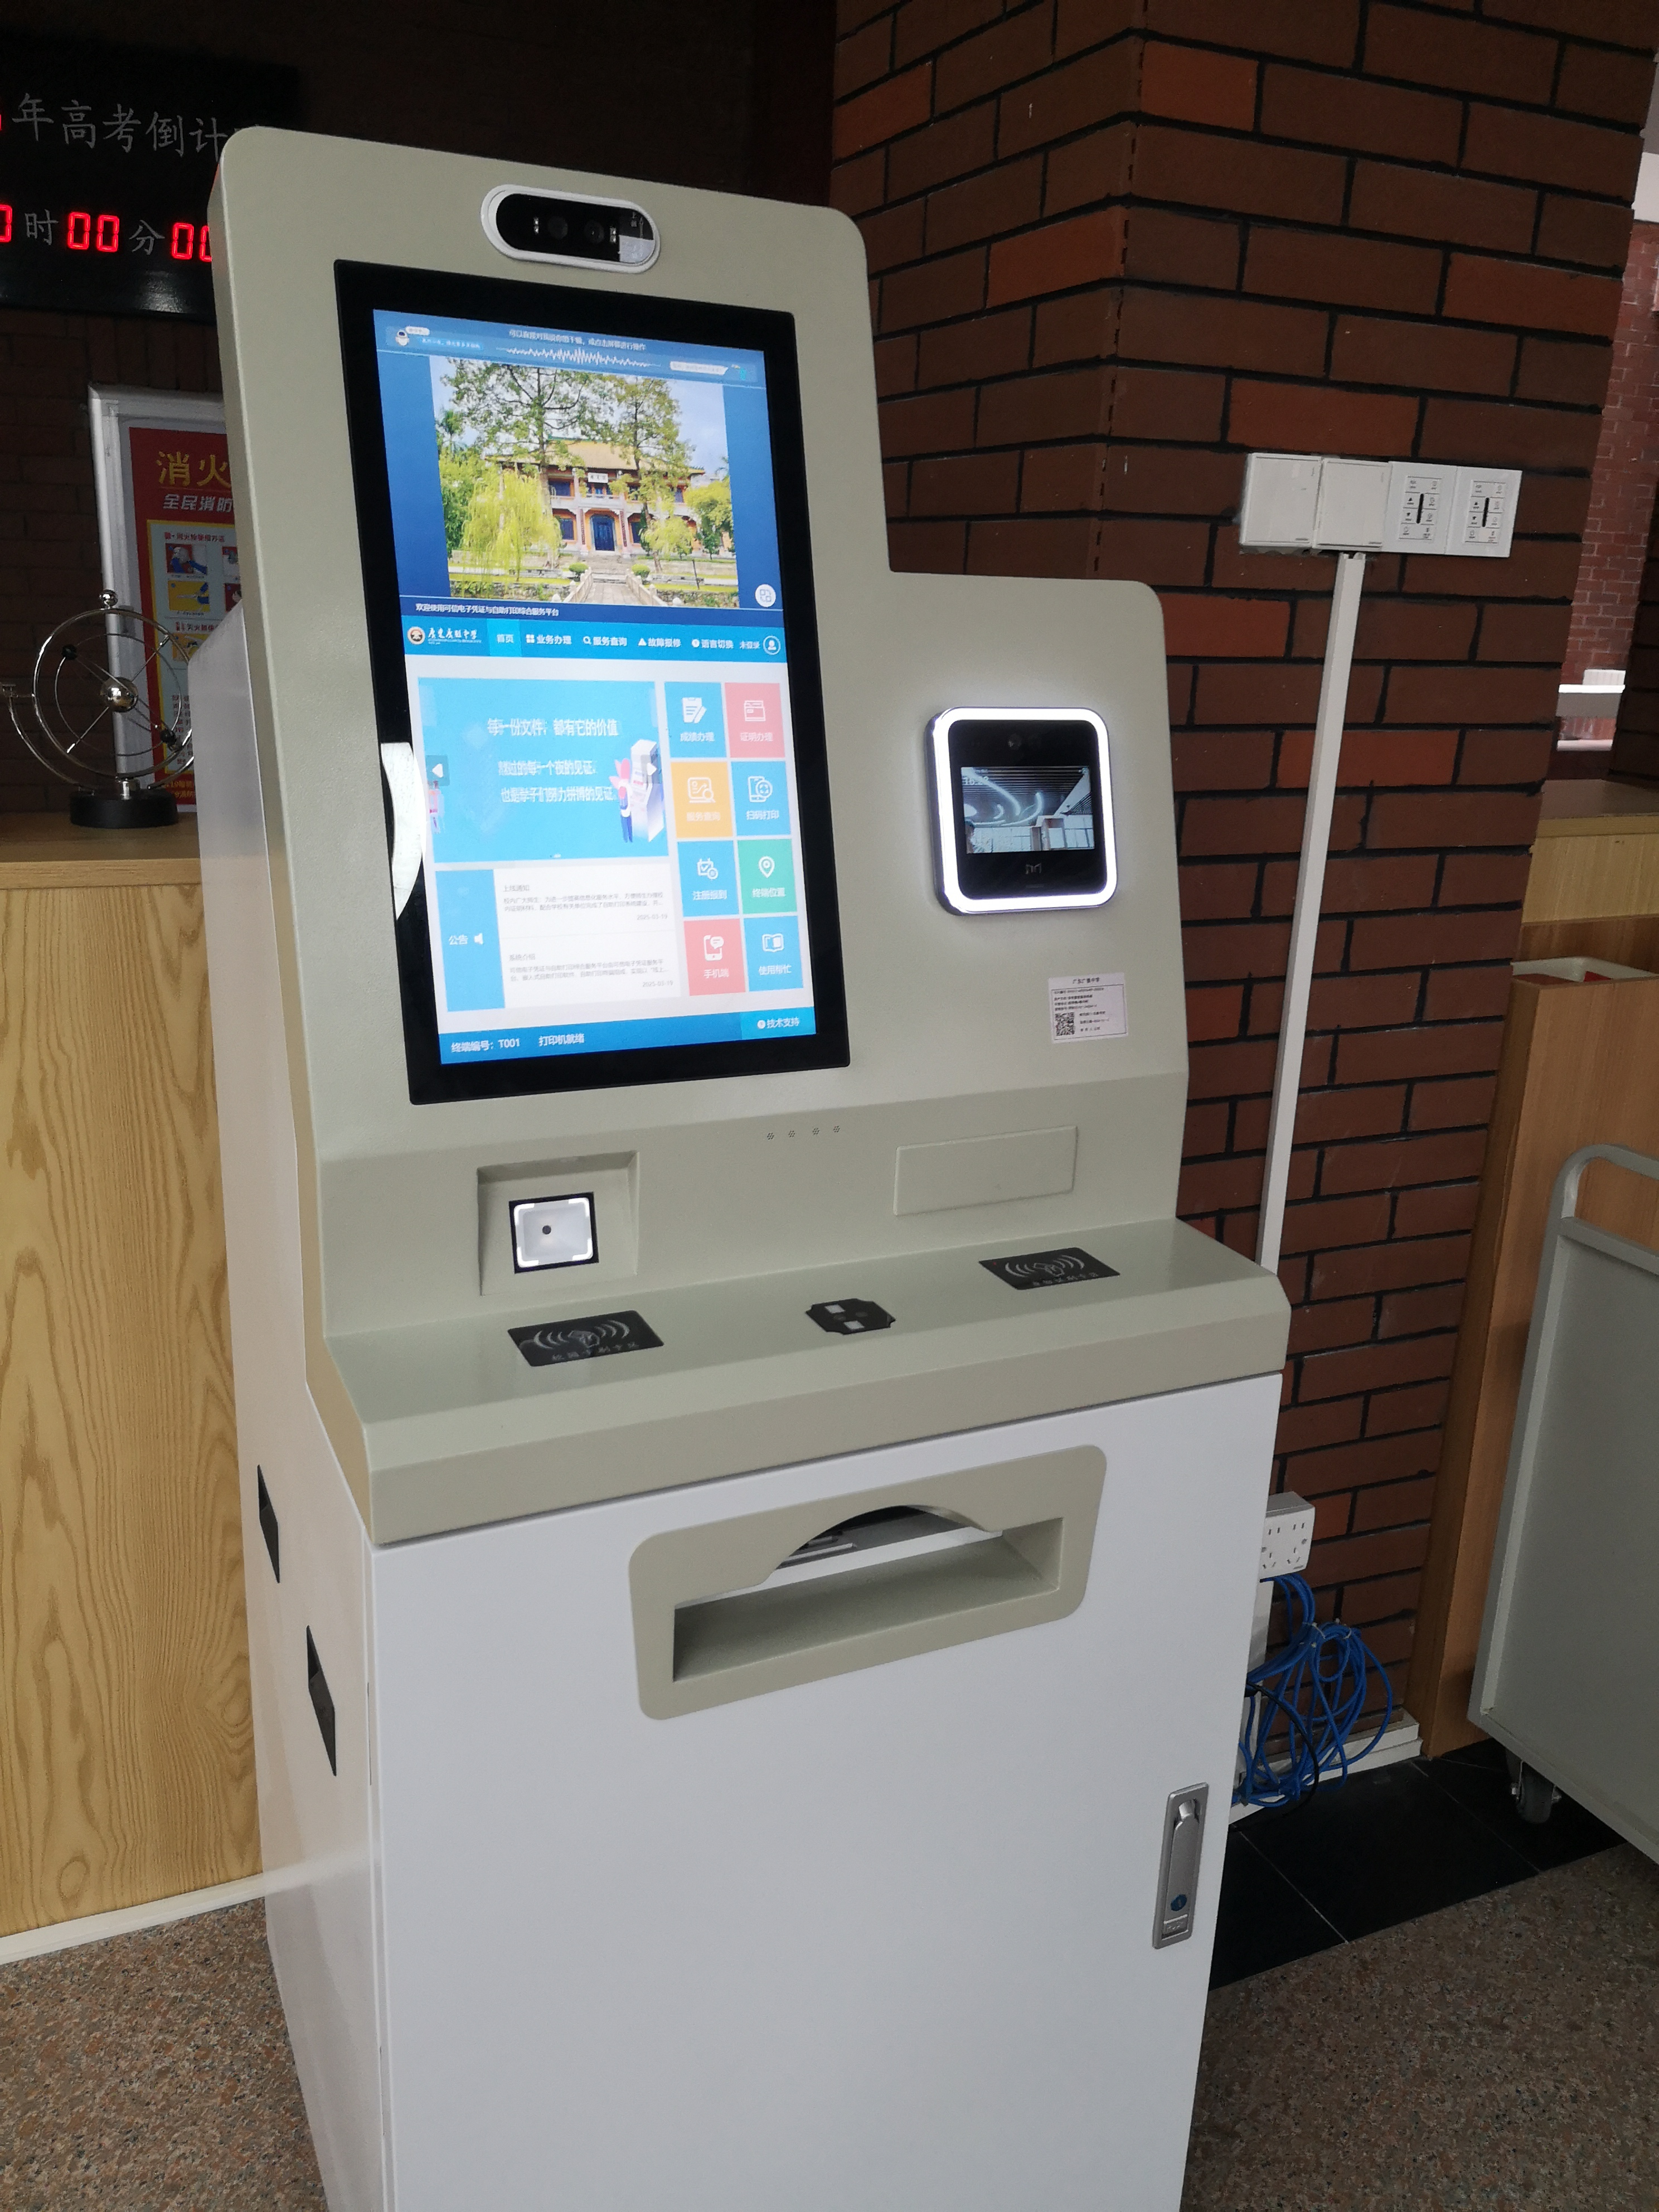
\includegraphics[width=\textwidth]{prove/prove1}
        \caption*{打印机}
        \label{fig:prove1}
      \end{minipage}
      \hfill
      \begin{minipage}{0.45\textwidth}
        \centering
        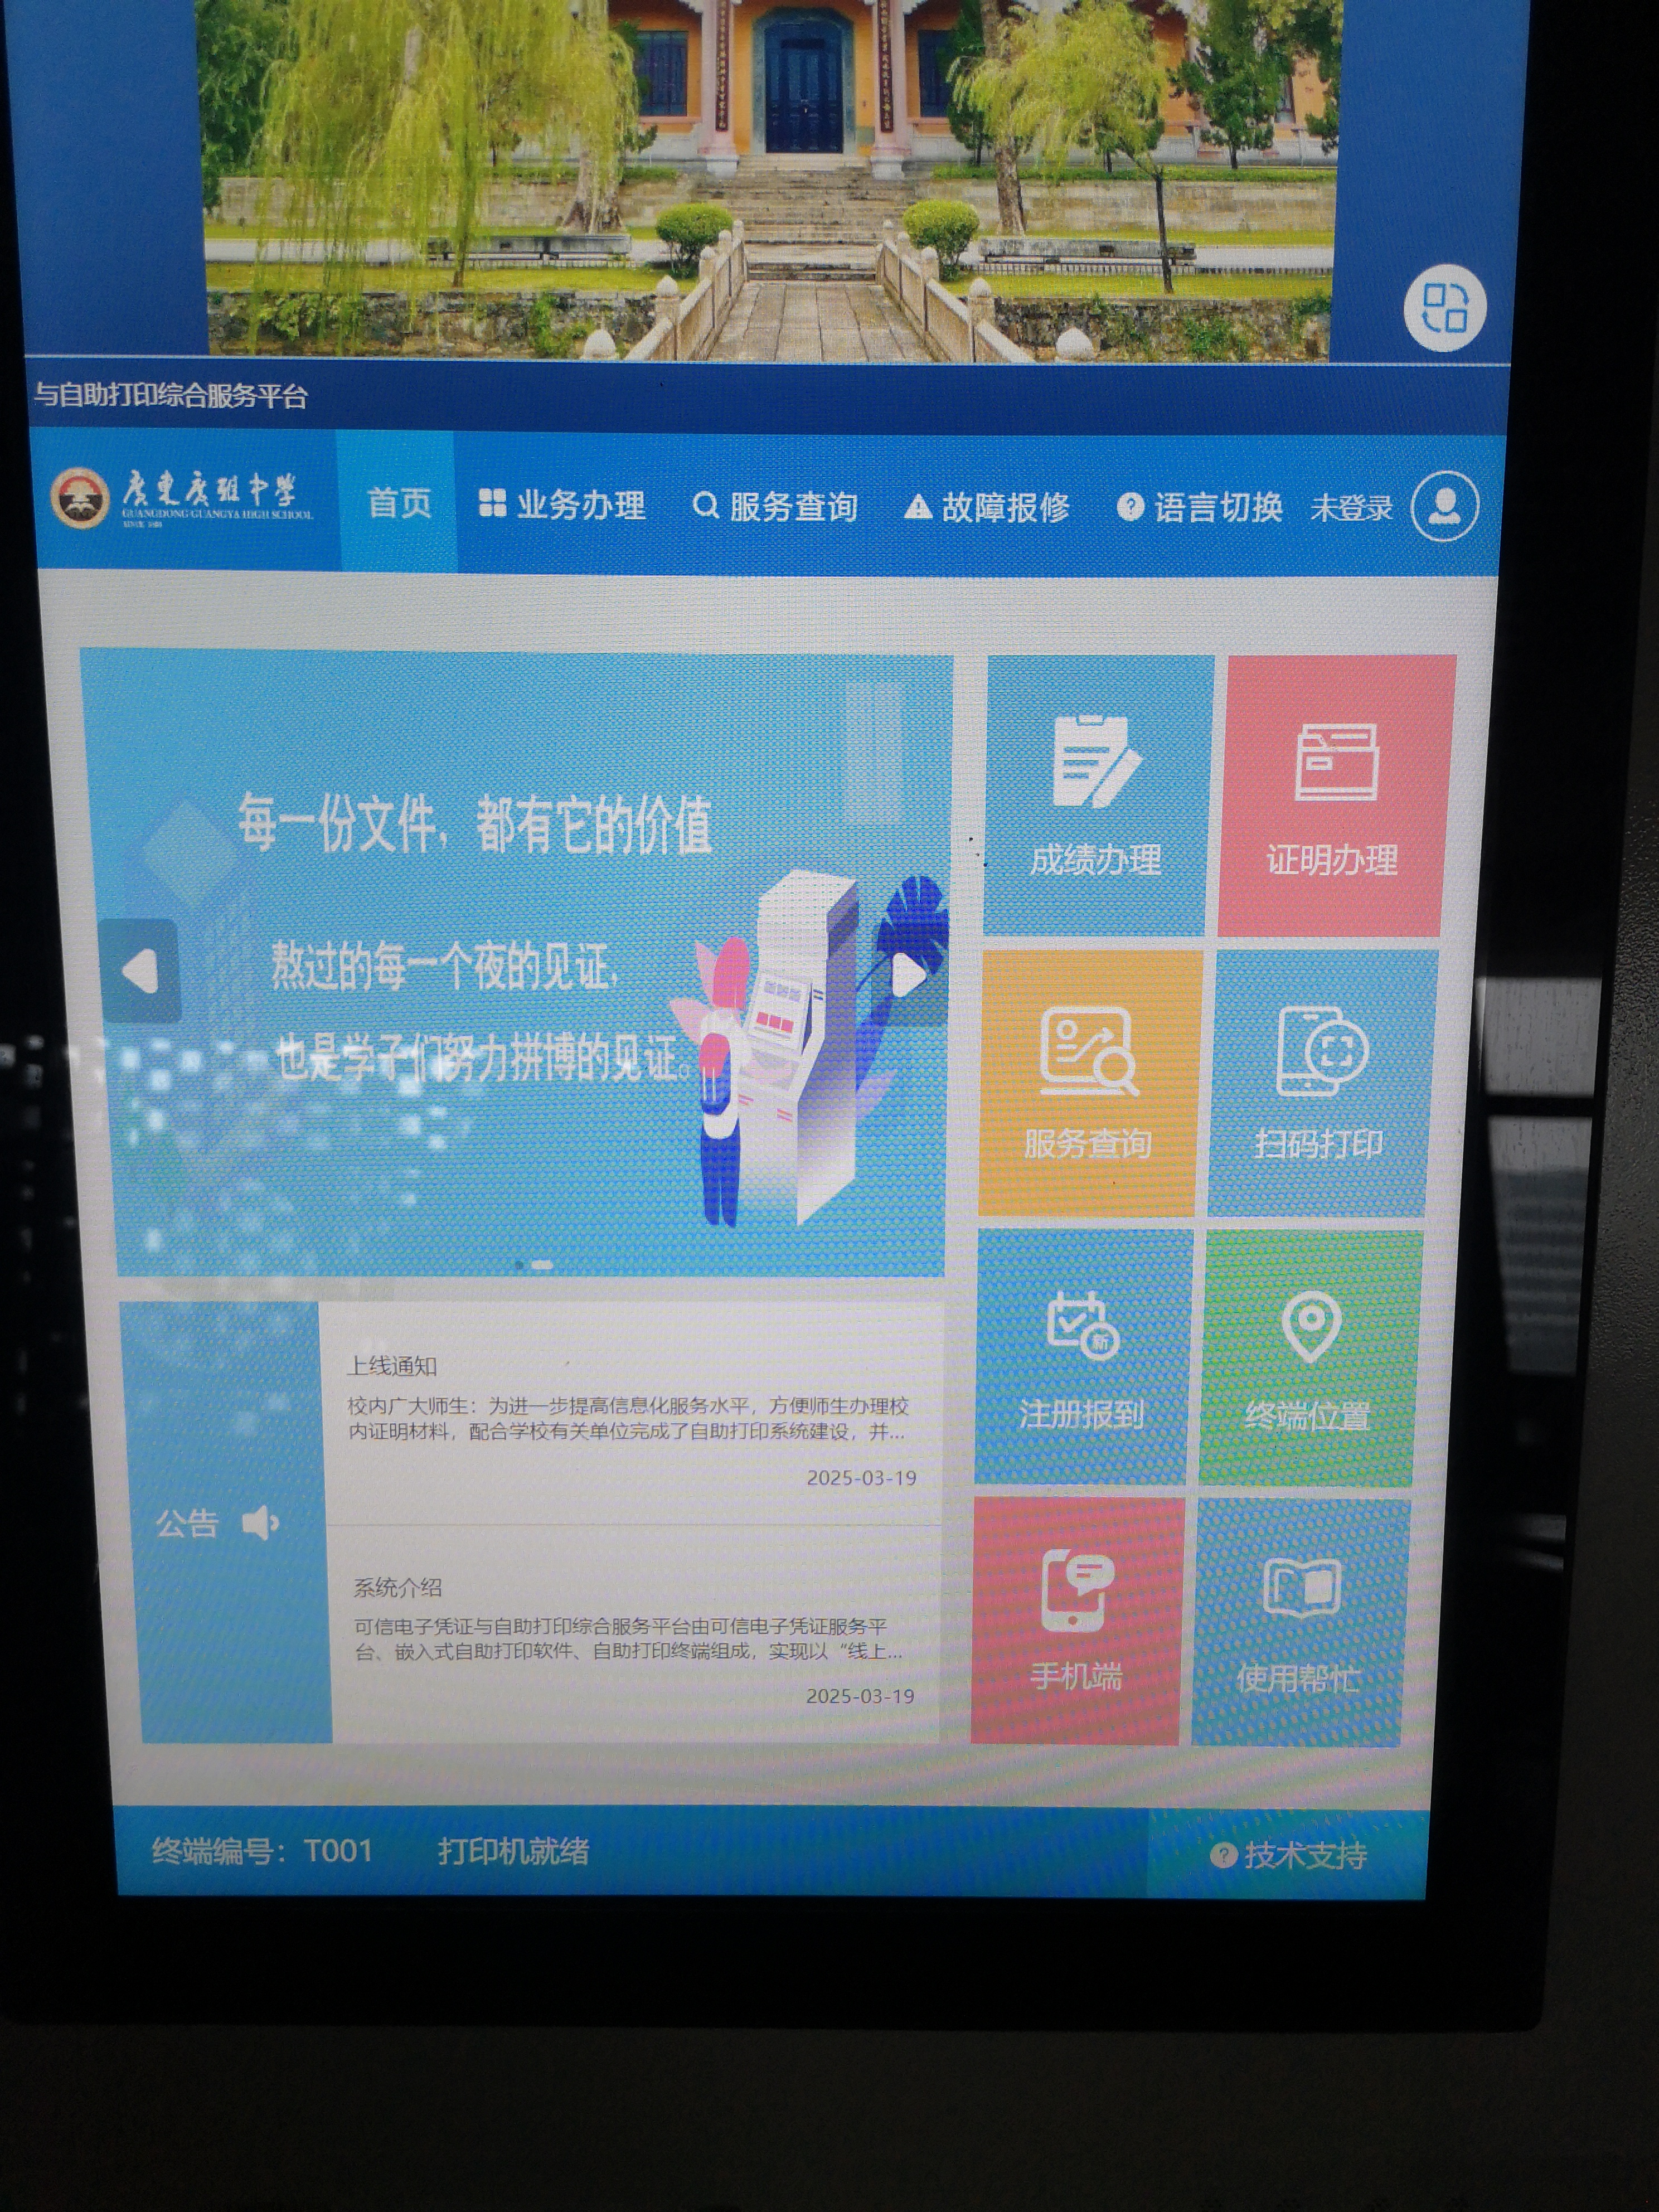
\includegraphics[width=\textwidth]{prove/prove2}
        \caption*{打印机屏幕}
        \label{fig:prove2}
      \end{minipage}
    \end{figure}
    我们可以点击右上角的“登录”来登录你的账号。什么？你不知道自己的账号是什么？没关系，点开后的登录方式选择“账号密码”，如\cref{prove3}。然后填写你的学号和身份证后6位，如\cref{prove4}。不出意外，没被别人改过得话，点击“登录”按钮就可以登录了。
    \begin{figure}[ht]
      \centering
      \begin{minipage}{0.45\textwidth}
        \centering
        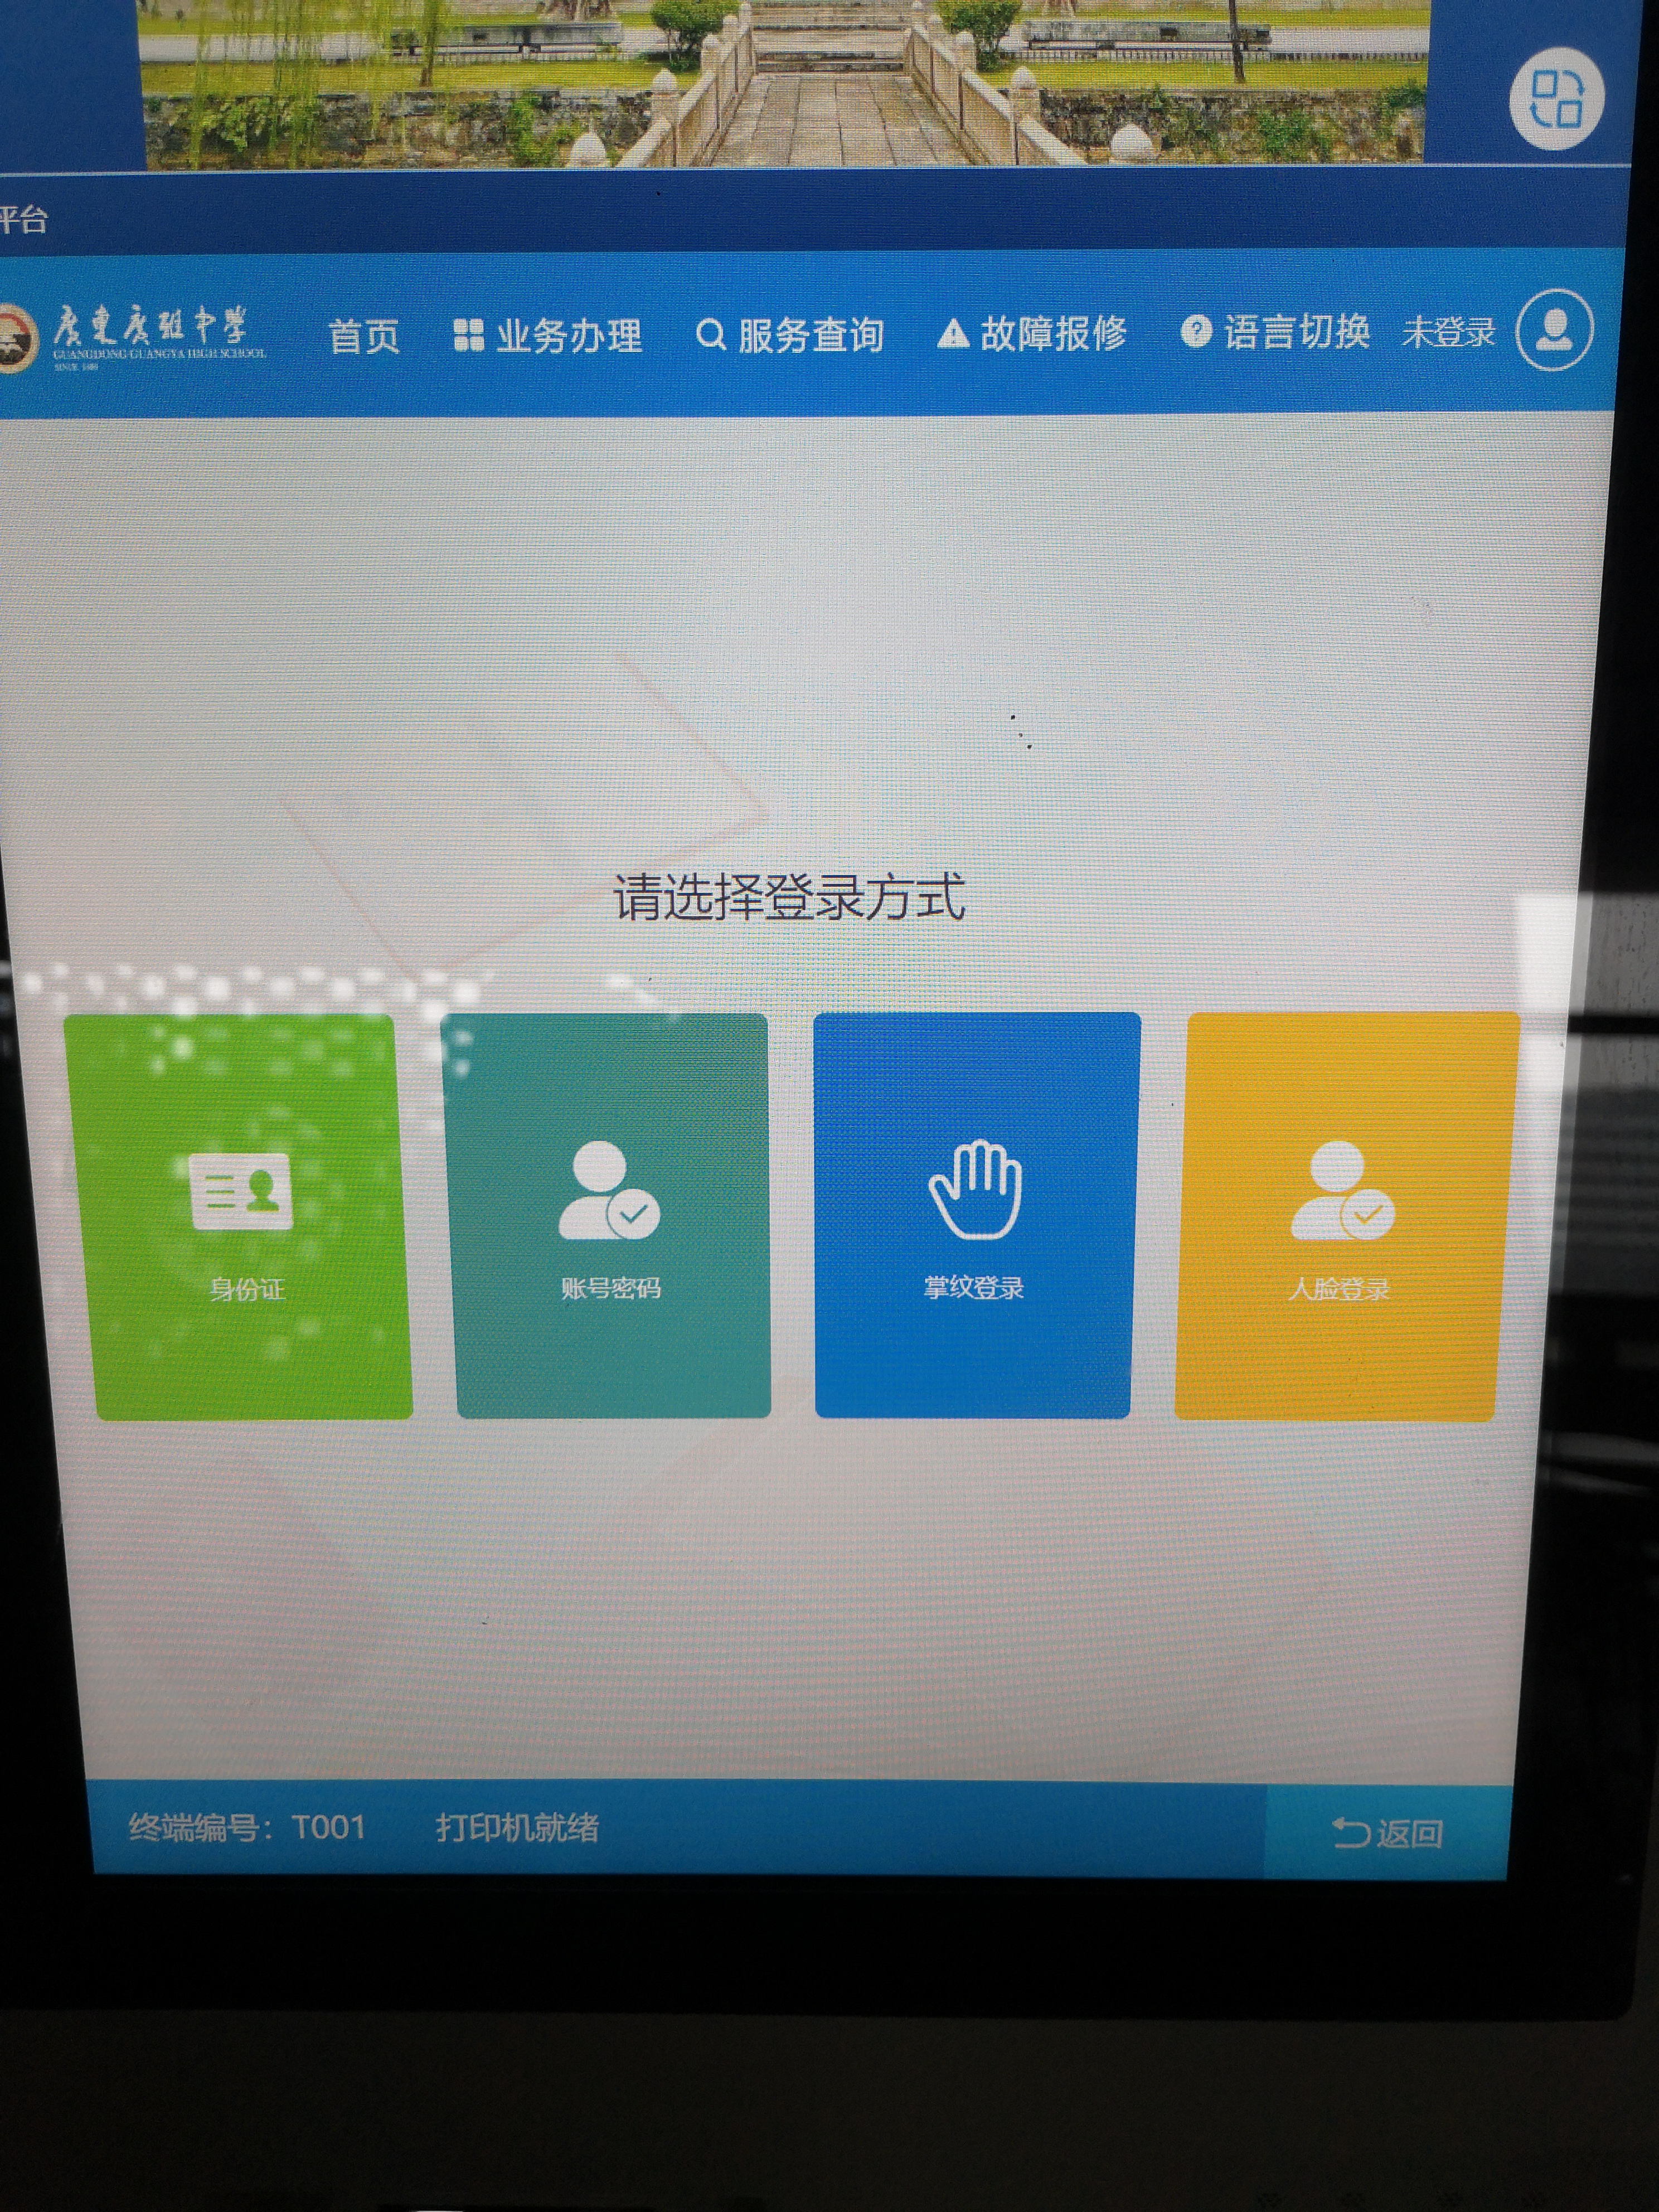
\includegraphics[width=\textwidth]{prove/prove3}
        \caption*{选择登录方式}
        \label{fig:prove3}
      \end{minipage}
      \hfill
      \begin{minipage}{0.45\textwidth}
        \centering
        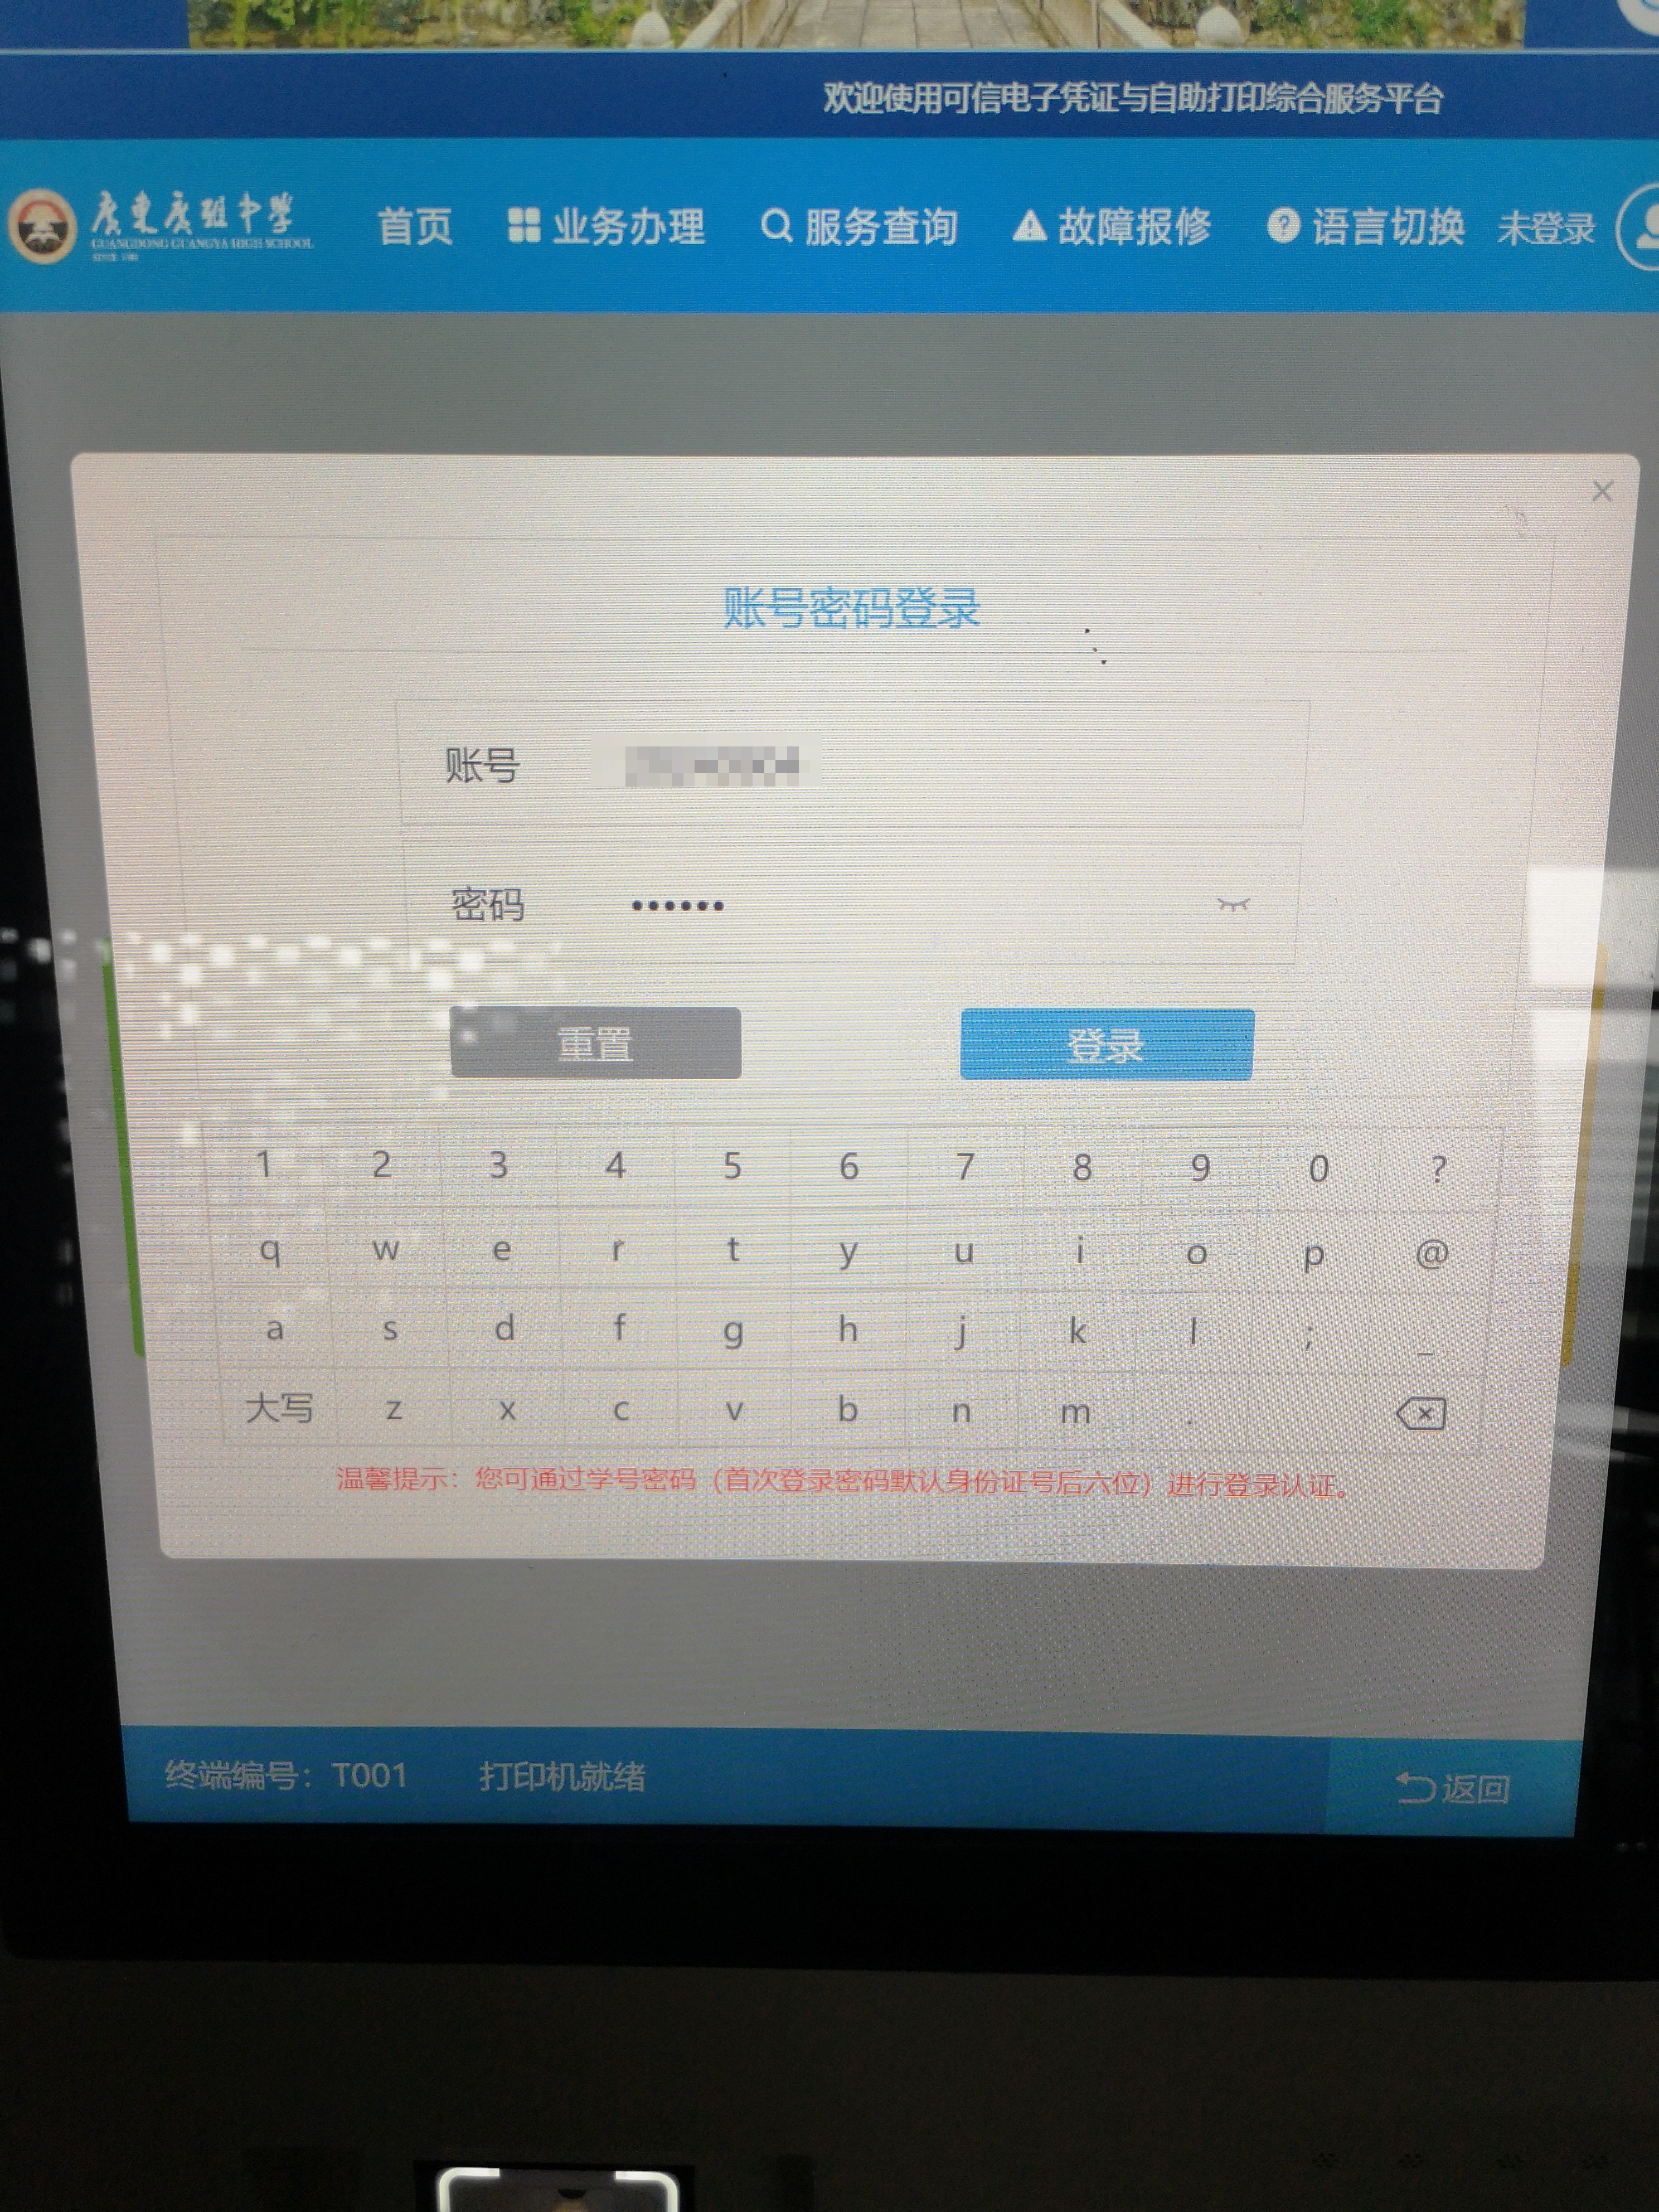
\includegraphics[width=\textwidth]{prove/prove4}
        \caption*{填写学号和身份证后6位}
        \label{fig:prove4}
      \end{minipage}
    \end{figure}
    然后，你就可以点击主页顶部菜单栏的“业务办理”，点击“中文成绩证明”，稍作等待，就能看到你的成绩证明了。
    \begin{figure}[ht]
      \centering
      \begin{minipage}{0.45\textwidth}
        \centering
        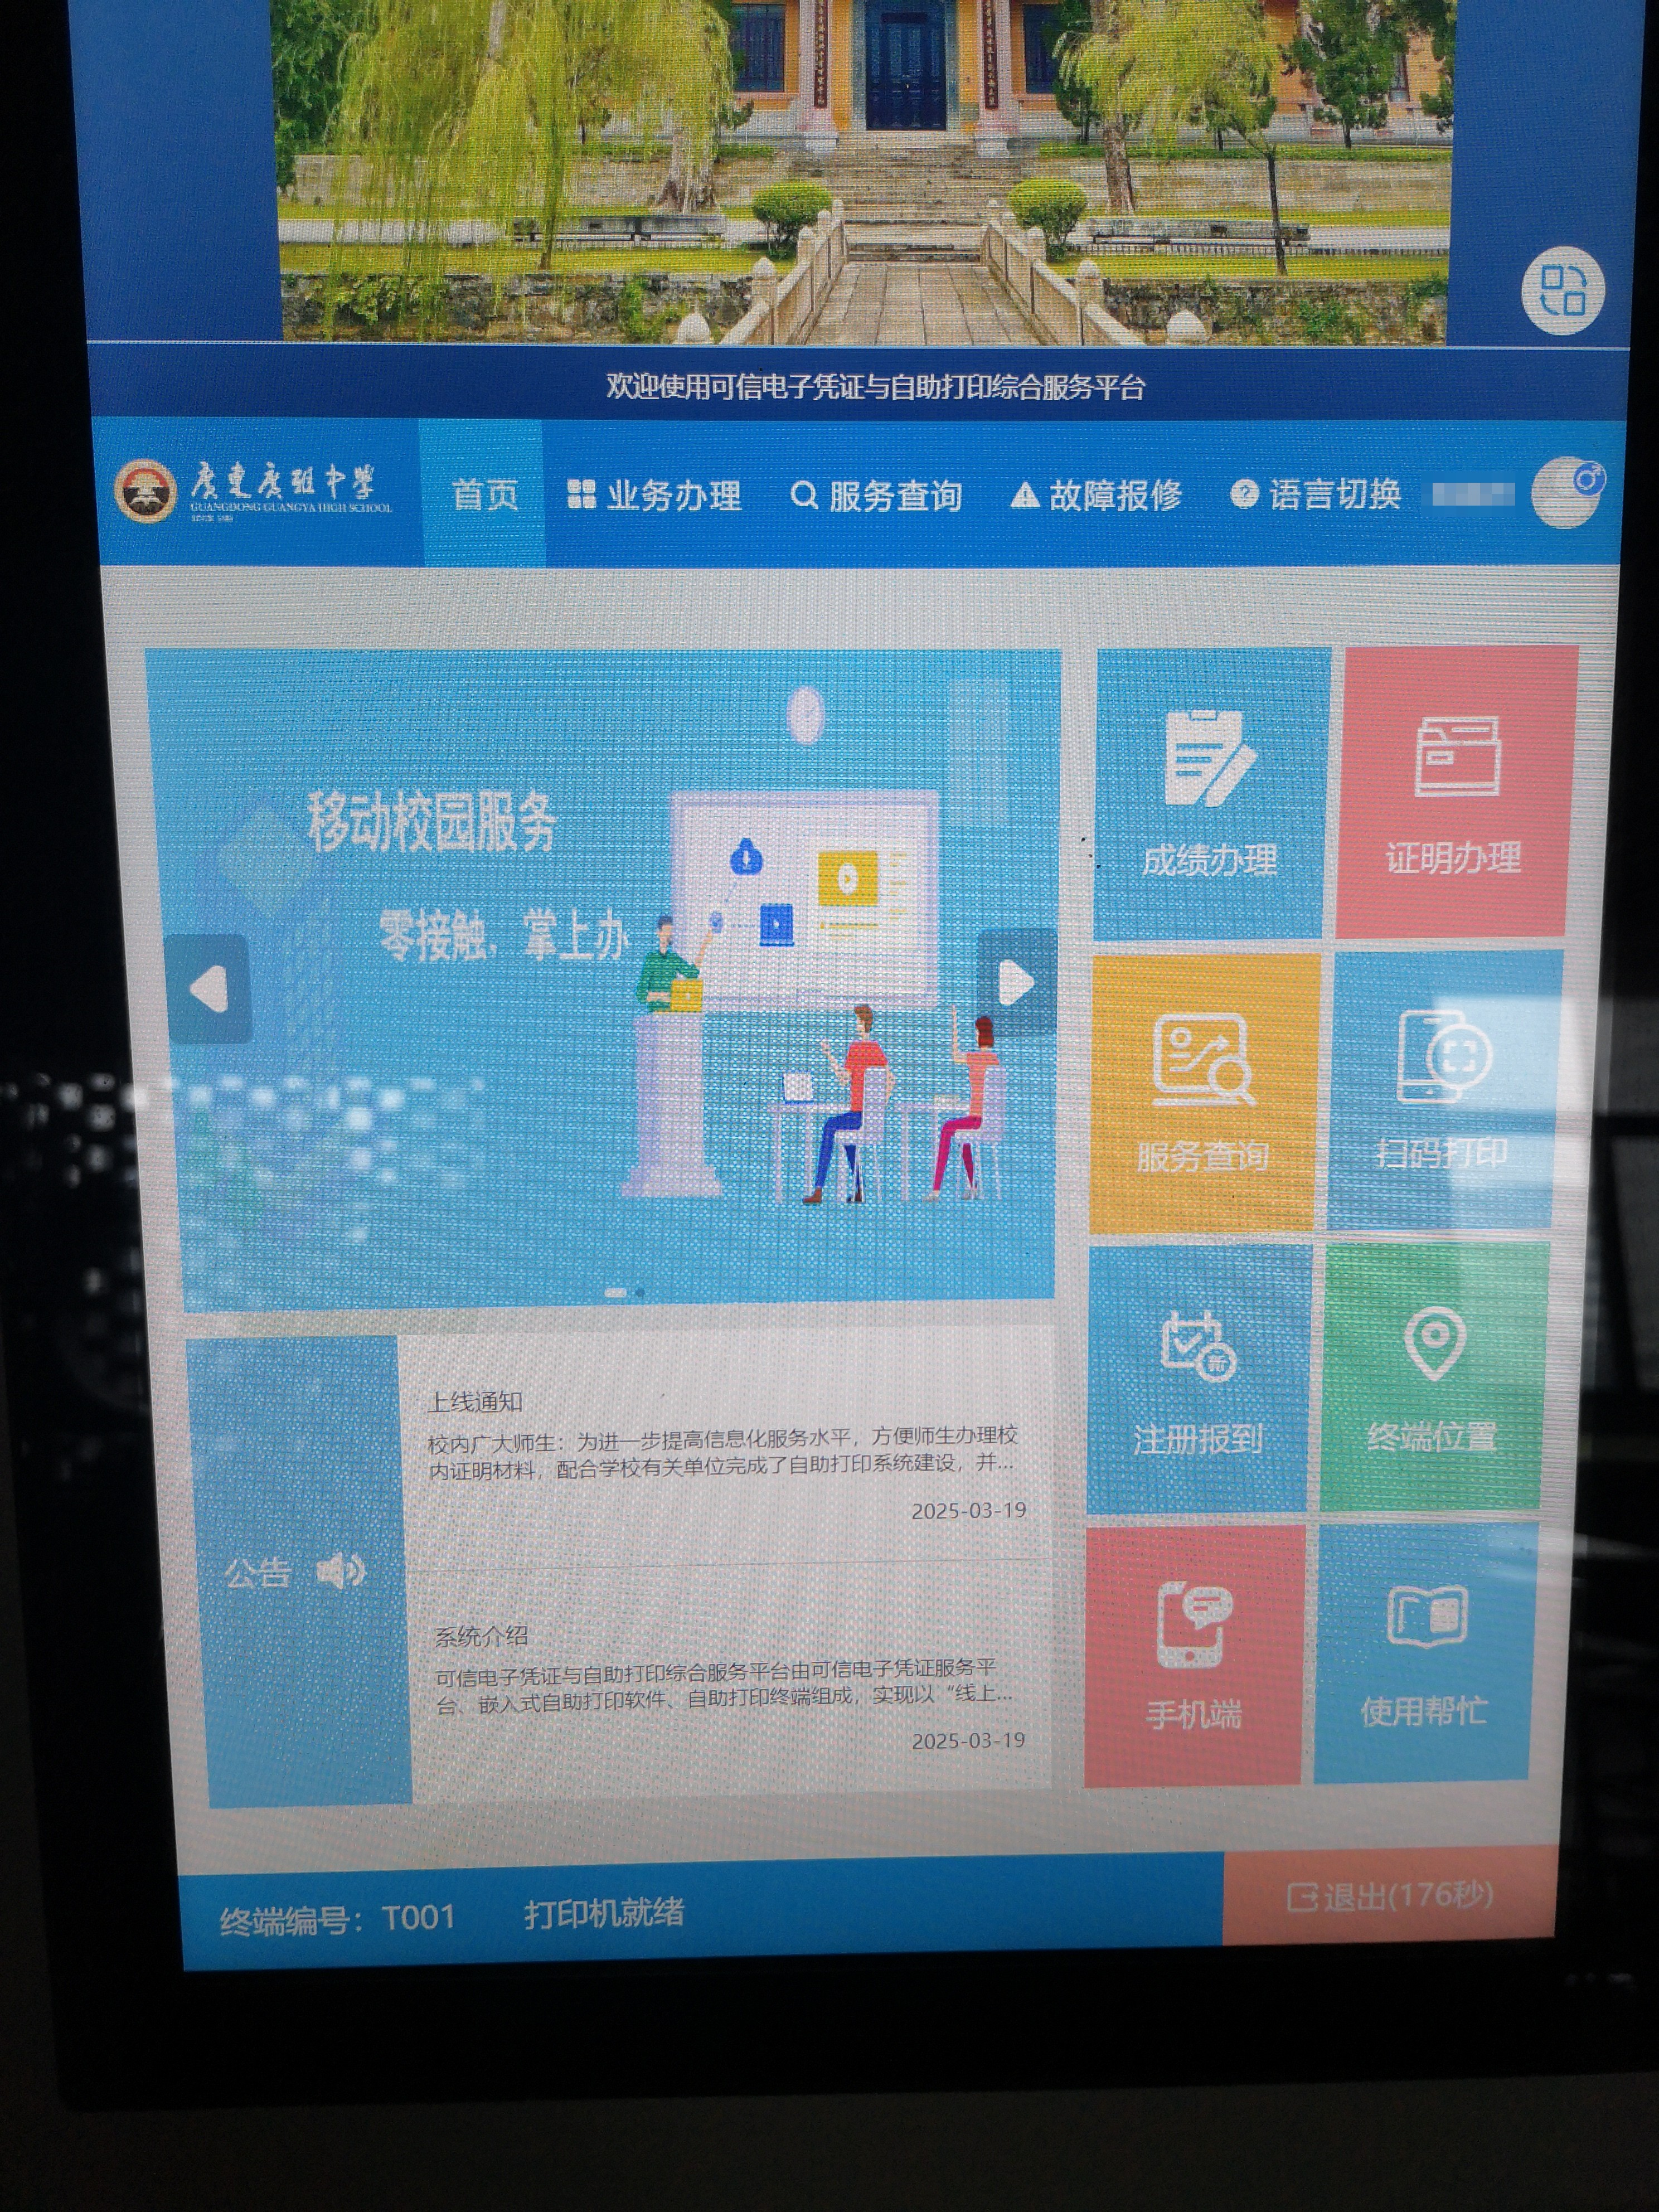
\includegraphics[width=\textwidth]{prove/prove5}
      \end{minipage}
      \hfill
      \begin{minipage}{0.45\textwidth}
        \centering
        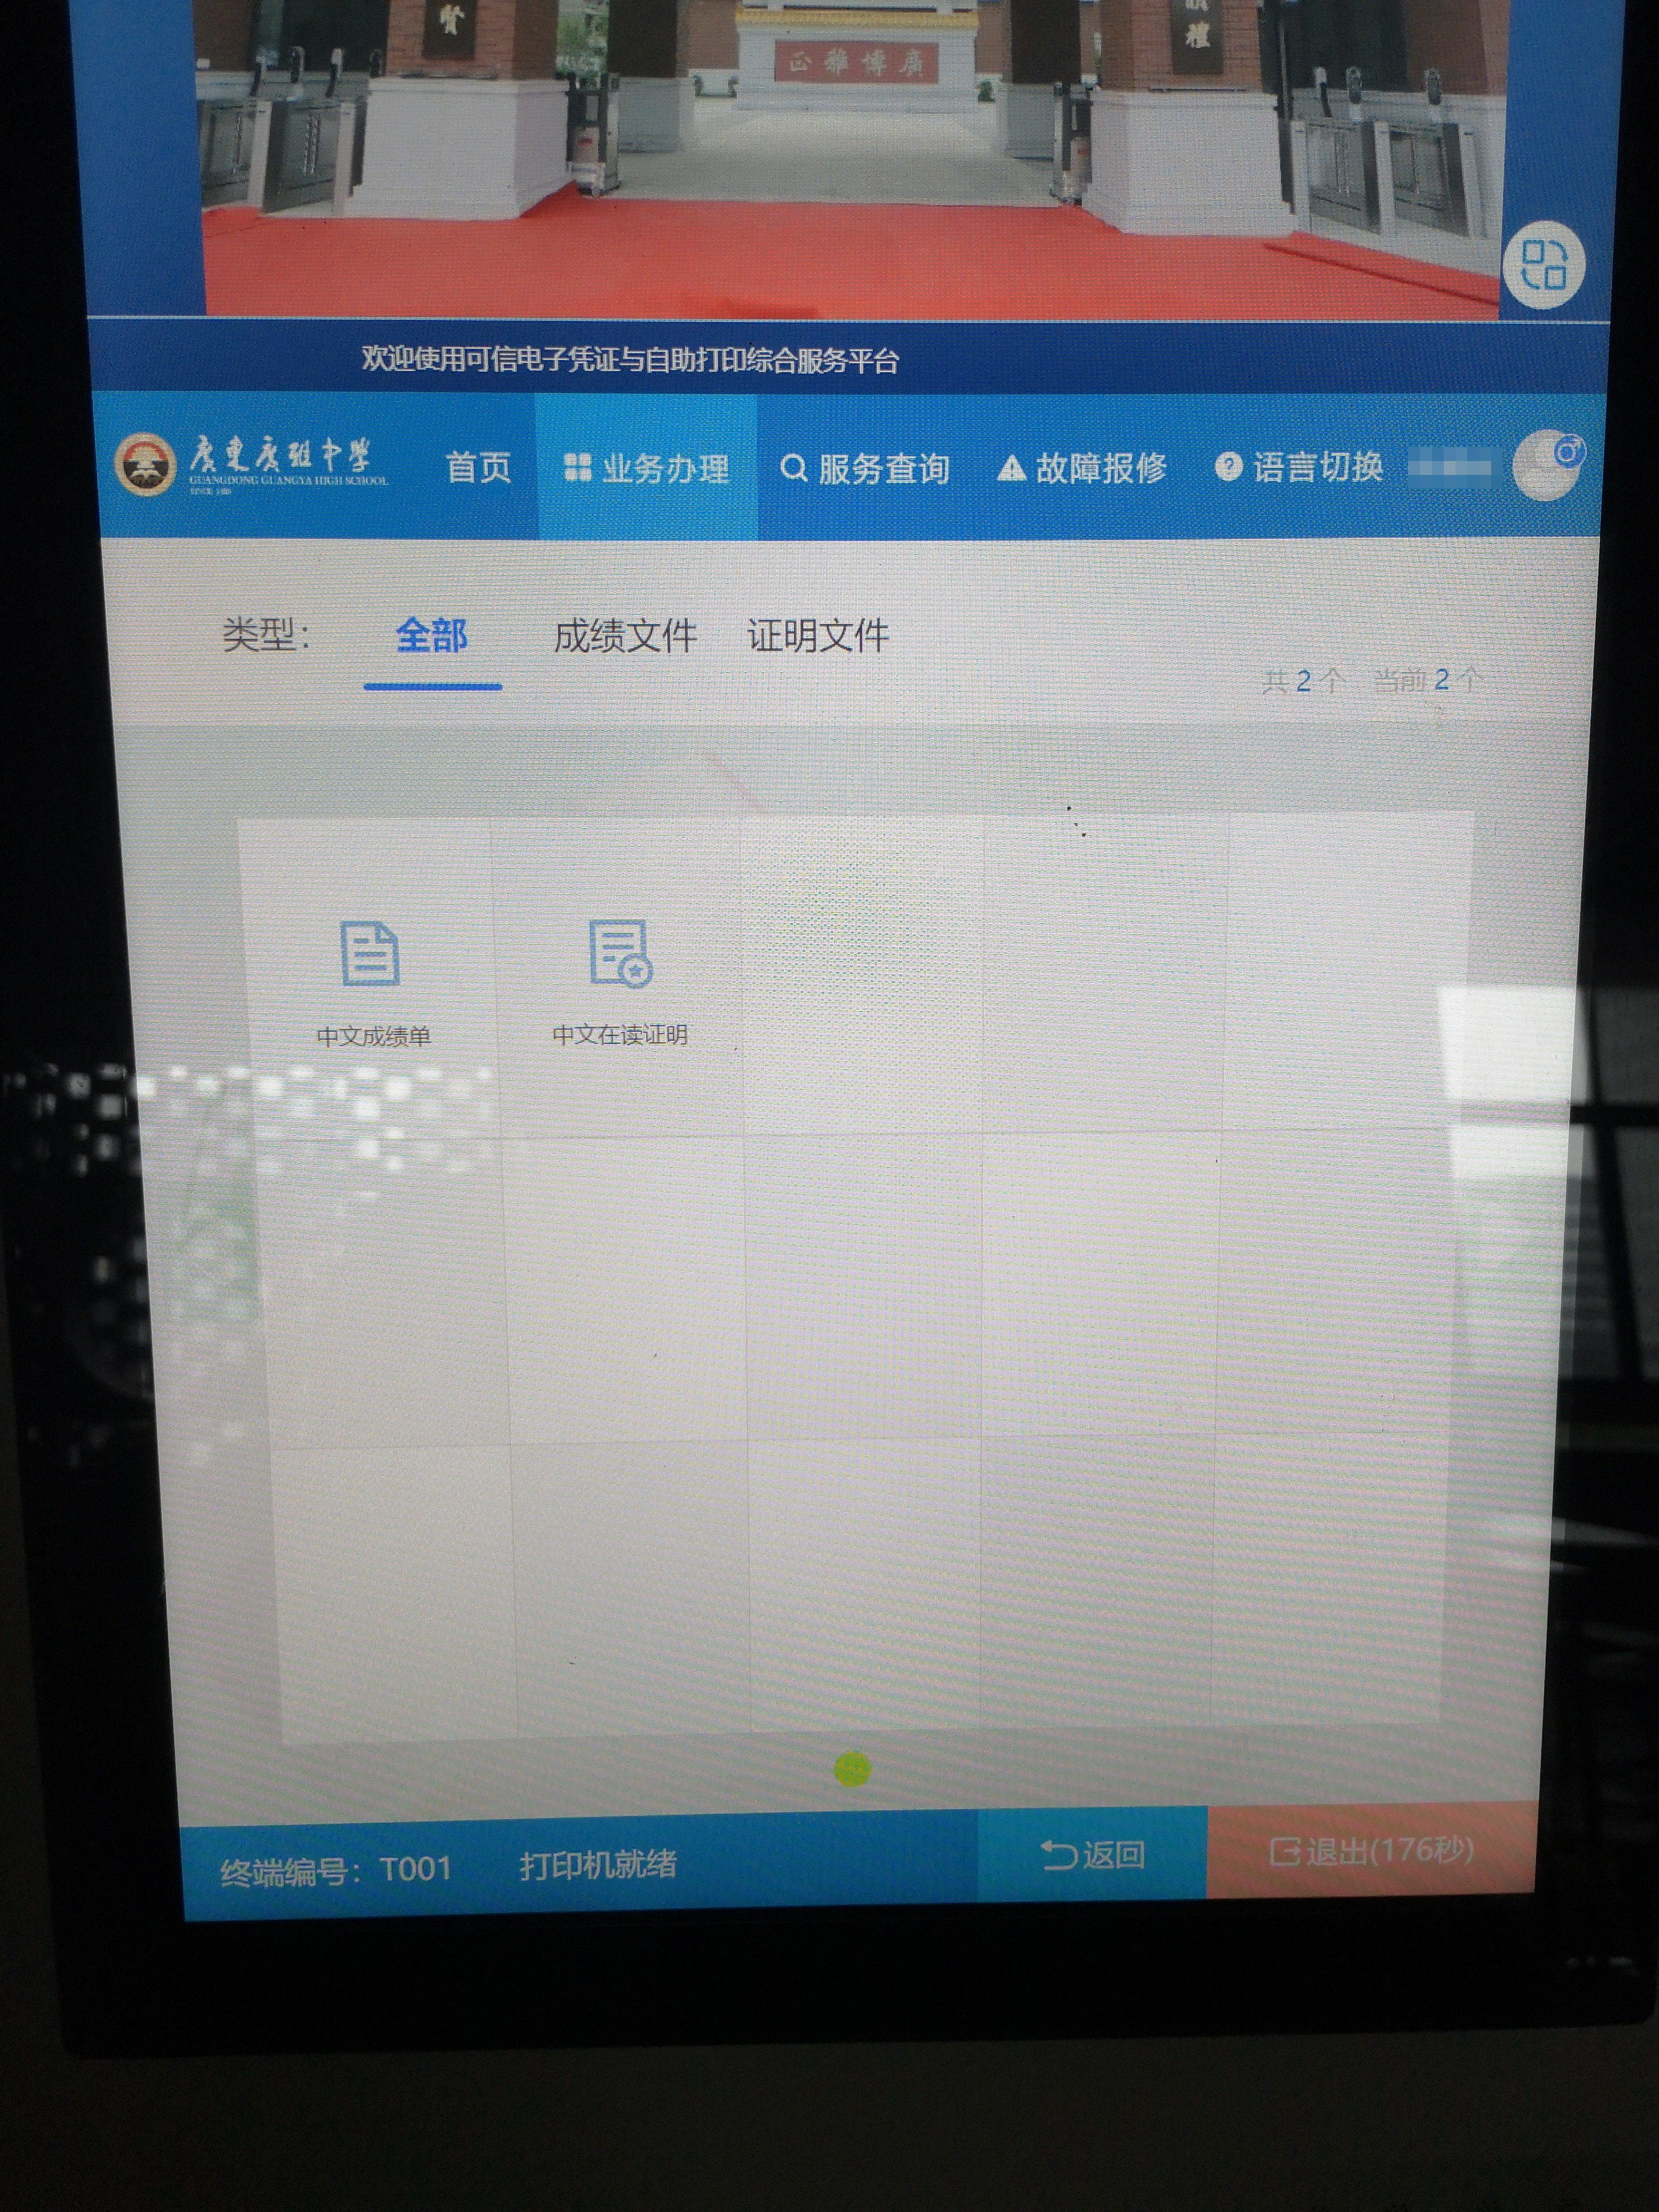
\includegraphics[width=\textwidth]{prove/prove6}
      \end{minipage}
      \caption{业务办理与中文成绩证明}
      \label{fig:prove56}
    \end{figure}
    然后，点击右边蓝色的打印机形状的按钮，就可以打印了，如\cref{fig:prove7}。每个学生可以免费打印10次。
    \begin{figure}[ht]
      \centering
      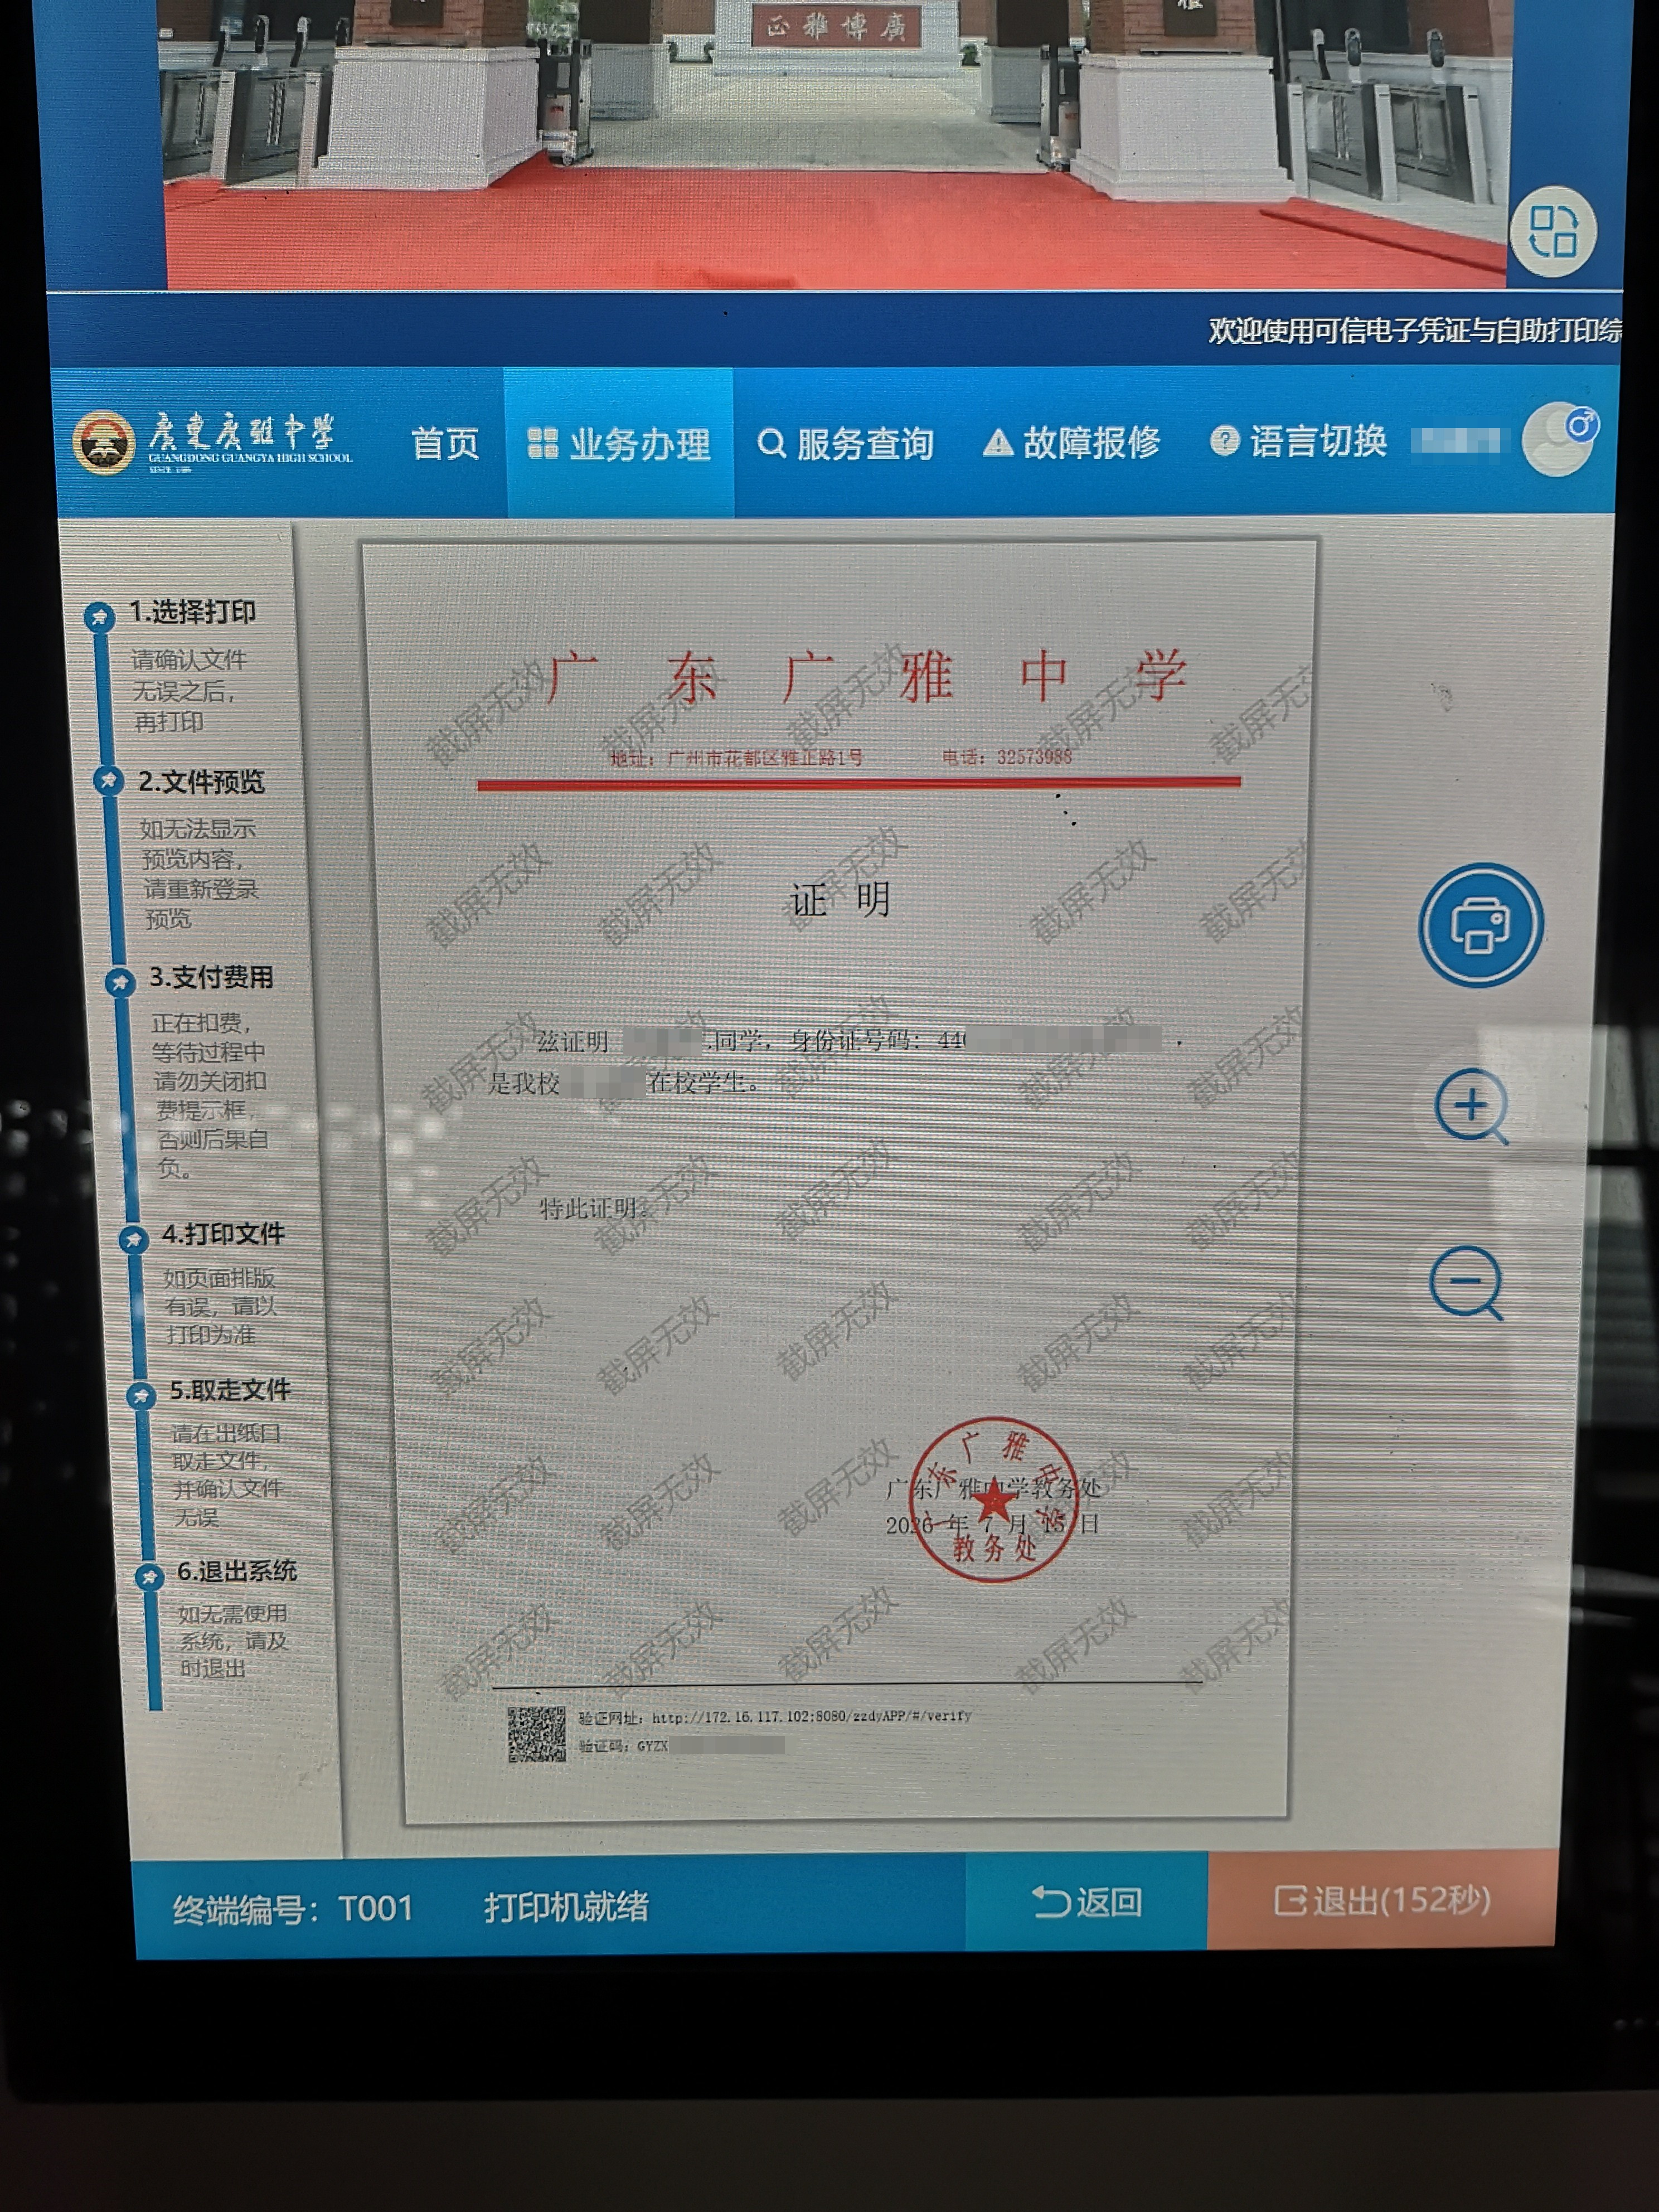
\includegraphics[width=0.45\textwidth]{prove/prove7}
      \caption{打印成绩证明}
      \label{fig:prove7}
    \end{figure}
    拿到打出来的纸质版成绩证明，就可以拿去尽情使用了。


\chapter{广雅的生活}
\label{chap:life}

  \section{饭堂}
  学生可用的饭堂共三层，分别有一楼、二楼东厅、二楼西厅、三楼东厅、三楼西厅。一般来说，一、二楼是普通餐，三楼是特色餐。中午的话，二楼*厅和一楼的饭菜是一样的。
  
  \section{宿舍}

\chapter{焚决}
\label{chap:secret}

教授一些小秘密^_^

\section{广雅应用}

先简单写一个从广雅应用到百度的超级无敌保姆级教程吧。首先你需要一个\emph{知乎账号}（重要），等广雅应用上来之后打开广雅应用
\begin{figure}[ht]
\centering
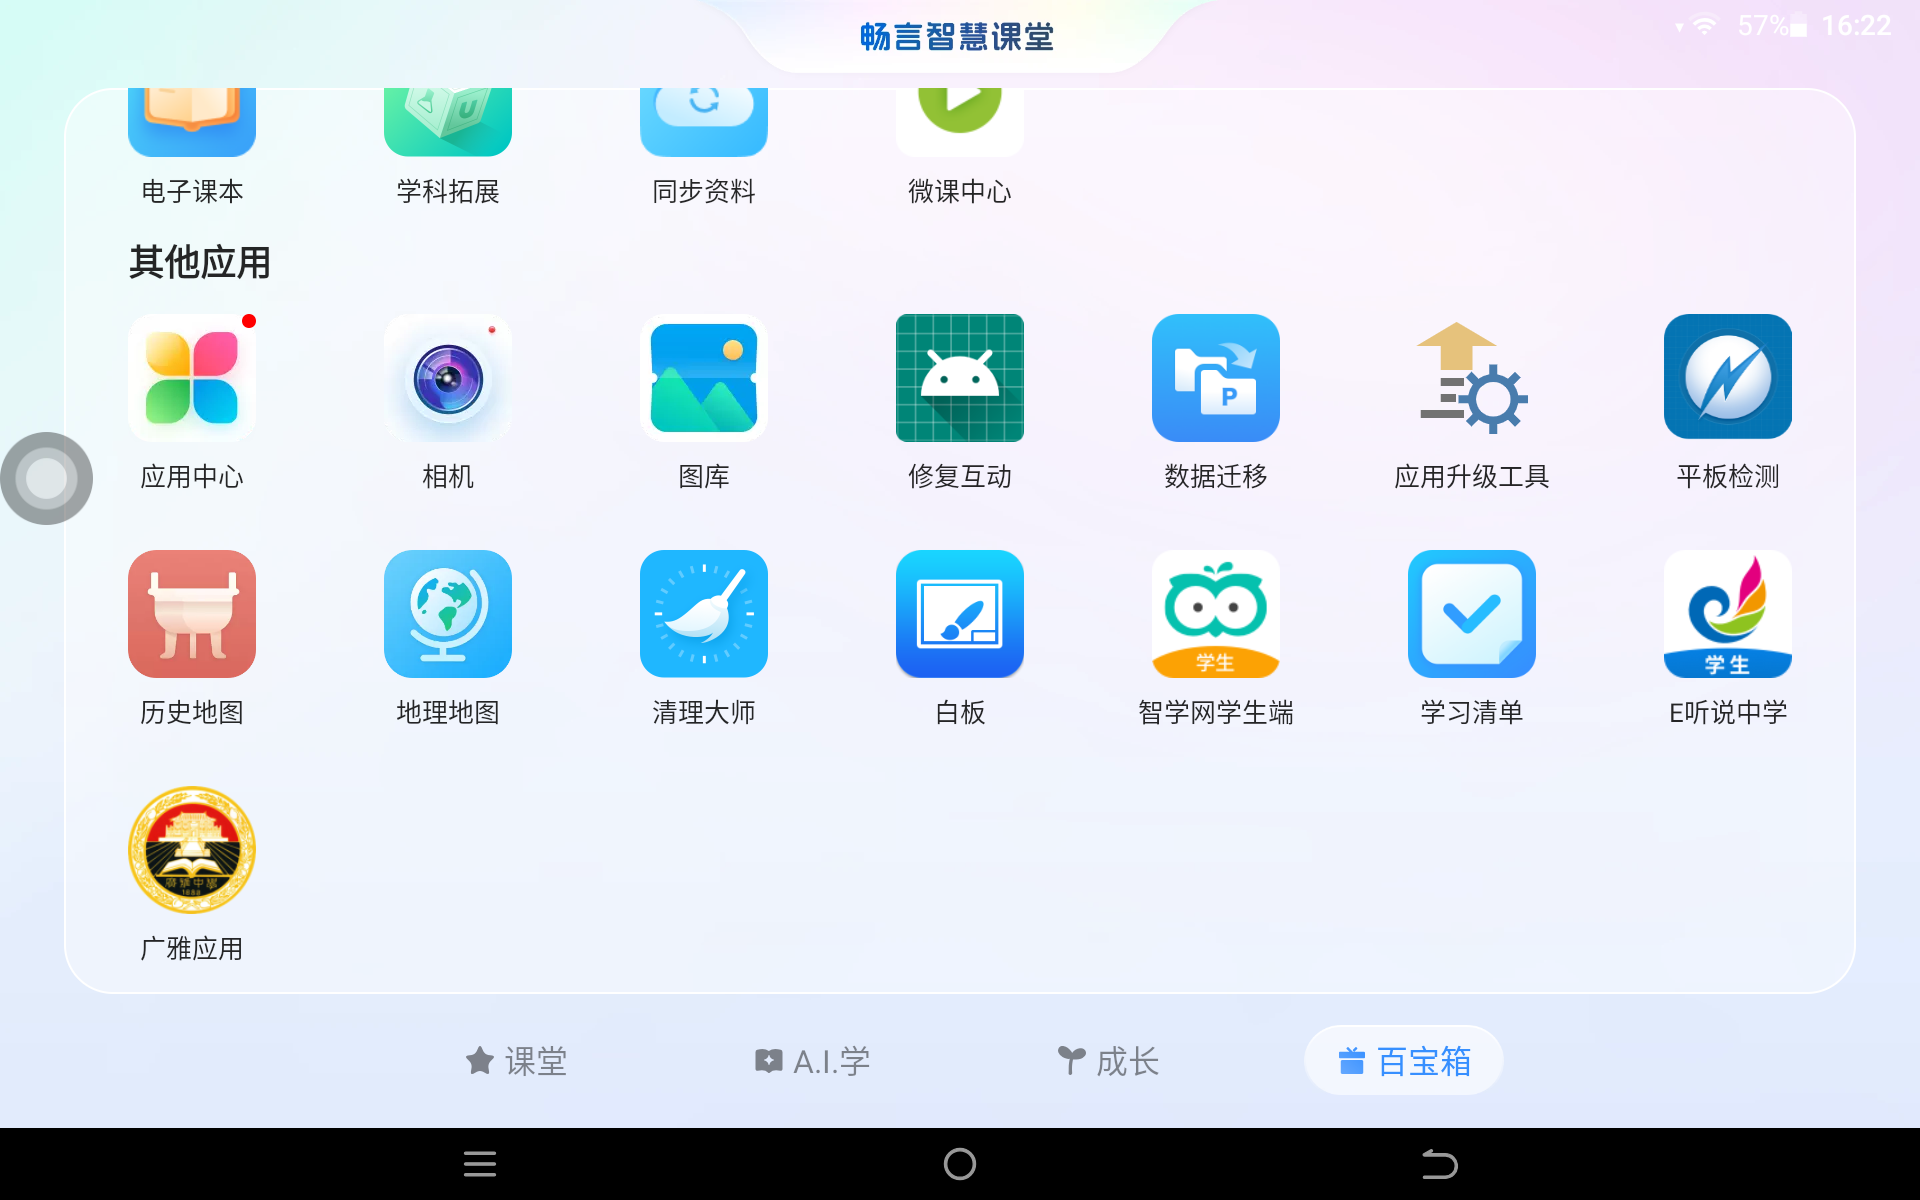
\includegraphics{../pics/toBaidu/1}
\caption{打开广雅应用}
\labrl{fig:openGY}
\end{figure}





\end{document}
